\section{Background}\label{s:background}

Before discussing the design and evaluation of the simulator, this section introduces the fundamental quantum concepts underlying the E91 key distribution protocol.

In E91, as in any quantum communication system, information is transmitted using \textbf{quantum states}. These states encode probability amplitudes whose squared magnitudes determine the likelihood of measurement outcomes. A quantum state that is expressed as a linear combination of basis states is said to be in a \textbf{superposition}.

The simplest representation of a quantum system is the \textbf{qubit}, a two-level quantum state defined in the computational basis as:
\[
\ket{0}, \quad \ket{1}.
\]

Using Born’s rule, the state of a qubit can be expressed as a linear combination of these basis states:
\[
\ket{\psi} = \alpha\ket{0} + \beta\ket{1},
\]
where $\alpha, \beta \in \mathbb{C}$ and satisfy the probability condition $|\alpha|^2 + |\beta|^2 = 1$.

To operate on qubits, we can use a set of quantum gates analogous to logic gates in classical computing. One example is the \textbf{Hadamard (H)} gate, which creates superposition states and is represented by the following matrix:
\[
H = \frac{1}{\sqrt{2}}
\begin{pmatrix}
1 & 1 \\
1 & -1
\end{pmatrix}.
\]

For multi-qubit systems, one of the most important gates is the \textbf{CNOT} (controlled-NOT) gate, which acts on a two-qubit system. Its matrix representation is given by:
\[
\mathrm{CNOT} =
\begin{pmatrix}
1 & 0 & 0 & 0 \\
0 & 1 & 0 & 0 \\
0 & 0 & 0 & 1 \\
0 & 0 & 1 & 0
\end{pmatrix}.
\]

Quantum states can also be represented as vectors in a complex Hilbert space. In this representation, the application of a quantum gate corresponds to matrix multiplication between the gate operator and the state vector.

In order to transform a qubit into a superposition state, where both measurement outcomes have equal probability, the Hadamard gate is applied to a qubit initially prepared in a computational basis state, such as $\ket{0}$.

Representing the basis state $\ket{0}$ as a vector:
\[
\ket{0} =
\begin{pmatrix}
1 \\
0
\end{pmatrix},
\]

we apply the Hadamard gate via matrix multiplication:
\[
H\ket{0}
=
\frac{1}{\sqrt{2}}
\begin{pmatrix}
1 & 1 \\
1 & -1
\end{pmatrix}
\begin{pmatrix}
1 \\
0
\end{pmatrix}
=
\frac{1}{\sqrt{2}}
\begin{pmatrix}
1 \\
1
\end{pmatrix}
=
\frac{1}{\sqrt{2}}(\ket{0} + \ket{1}).
\]


\textbf{Entanglement}, a key aspect of the E91 protocol, occurs when two qubits are prepared in a quantum state such that their measurement outcomes exhibit correlations, regardless of distance. These entangled two-qubit states are known as Bell states, named after physicist John Bell, who developed Bell’s theorem to test the non-classical nature of such correlations.

One of the four maximally entangled two-qubit Bell states is defined as:
\[
\ket{\Phi^{+}} = \frac{1}{\sqrt{2}}(\ket{00} + \ket{11}), \quad
\]

% Explain how entanglement is produced via CNOT gates
  %% Show the matrix equatios
In order to produce a Bell state, you first apply a Hadamard gate, followed by a CNOT gate.

When both qubits of the Bell state are measured in the same basis, the outcomes are perfectly correlated, giving identical results (either 00 or 11) despite each result being individually random. This basis-dependent correlation is the key resource exploited in the E91 protocol, enabling both key generation and eavesdropping detection through later comparison of measurement outcomes.

Building on these quantum mechanical principles, the E91 protocol enables two nodes in the quantum internet, to establish a shared secret key using entangled qubit pairs distributed by a quantum source.

E91 relies on the distribution of entangled states, typically Bell states, such that correlations between measurement outcomes can be used both for key generation and for detecting the presence of an eavesdropper.

In the standard setting, a trusted, usually refered as epr node, distributes entangled qubit pairs to both of the client nodes over a quantum channel. Each party independently measures their qubits using randomly chosen measurement bases. The choice of measurement basis plays a central role in both the generation of the key and the security analysis of the protocol.

\begin{figure}[h]
    \centering
    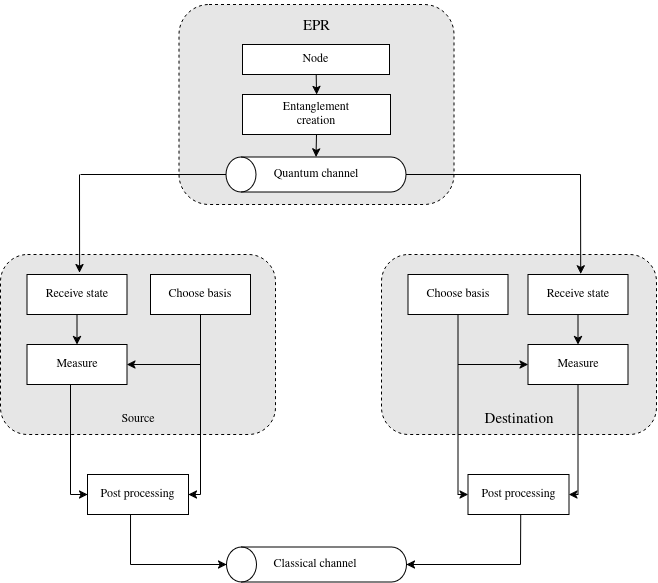
\includegraphics[width=0.5\textwidth]{../figures/E91.png}
    \caption{Diagram describing E91 process}
    \label{fig:E91}
\end{figure}

Once all entangled pairs have been distributed and measured, both nodes share their chosen measurement bases over a classical channel, which reveals little to no useful information to an eavesdropper.

Using this basis information, the measured qubits can be divided into two groups:

\begin{itemize}
  \item \textbf{Key qubits}: These correspond to measurements where both parties used the same basis. Assuming ideal entanglement and no fidelity loss, the resulting measurement outcomes should be perfectly correlated.

  \item \textbf{Test qubits}: These correspond to measurements performed in different bases. These outcomes are used to evaluate quantum correlations and to detect the presence of an eavesdropper in the communication channel.
\end{itemize}

In the E91 protocol, the measurement bases correspond to rotations on the Bloch sphere that define the detector settings used to measure incoming qubits. Following \cite{guimaraes2024bells}, the choice of measurement angles that maximizes quantum correlations and leads to a strong violation of the Bell inequality must be chosen in steps of $\frac{\pi}{8}$. The ones chosen for this simulator were: 
\begin{align*}
\alpha &= 0 \quad (0^\circ), \qquad \alpha' = \frac{\pi}{4} \quad (45^\circ), \\
\beta &= -\frac{\pi}{8} \quad (-22.5^\circ), \qquad \beta' = \frac{\pi}{8} \quad (22.5^\circ),
\end{align*}
where $\alpha, \alpha'$ correspond to one party's polarizer settings and $\beta, \beta'$ correspond to the other party's polarizer settings. 

The CHSH test is an experimental test of Bell's theorem, which shows that no physical theory based on local hidden variables can reproduce all predictions of quantum mechanics.

This result is expressed using the CHSH $S$-parameter \cite{shafi2021}, defined as 
\[
S = \left|E(A_0, B_0) + E(A_0, B_1)\right| + \left|E(A_1, B_0) - E(A_1, B_1)\right|.
\]

Here, $E(A_i, B_j)$ denotes the expectation value of the correlation between measurement settings $A_i$ and $B_j$.

In any local hidden variable theory, the CHSH inequality imposes the bound
\[
S \le 2,
\]
whereas quantum mechanics predicts a stronger limit,
\[
S \le 2\sqrt{2}.
\]

Based on \cite{vanHee2026} when the basis are used as polarizer angles (moving the detector by such an angle) the expectation value can be calculated as: 

$$
E(a,b) = \cos\big(2(a-b)\big)
$$

%% TODO: Give the functions numbers
Therefore, the CHSH value for our choice of basis is given by
\[
E(\alpha,\beta)=\cos\left(\frac{\pi}{4}\right)=\frac{\sqrt{2}}{2}, \quad
E(\alpha,\beta')=\cos\left(-\frac{\pi}{4}\right)=\frac{\sqrt{2}}{2},
\]
\[
E(\alpha',\beta)=\cos\left(\frac{3\pi}{4}\right)=-\frac{\sqrt{2}}{2}, \quad
E(\alpha',\beta')=\cos\left(\frac{\pi}{4}\right)=\frac{\sqrt{2}}{2}.
\]

Substituting into the CHSH expression,
\[
S = \left|E(\alpha,\beta)+E(\alpha,\beta')\right|
+ \left|E(\alpha',\beta)-E(\alpha',\beta')\right|,
\]
gives
\[
S = \left|\sqrt{2}\right| + \left|-\sqrt{2}\right| = 2\sqrt{2}.
\]

If after calculating the S parameter, we get $\left|S\right| < 2$, we can assume that the correlation is not maximal and there is a third person in the communication

% Explain Cascade error correction
The Cascade protocol functions as a multi-pass block-parity check designed to reconcile bit errors between Alice and Bob caused by fidelity loss. In the first pass, the sifted bit strings are divided into equal-sized blocks ($k_1$), and Alice transmits the parity of each block to Bob. For any block where parities disagree—signaling an odd number of errors—the parties execute the BINARY subprotocol. This subprotocol bisects the block and compares the parities of the halves until the exact position of a single erroneous bit is isolated and corrected by Bob, leaving all remaining blocks with an even number of errors.

In subsequent passes ($i > 1$), the block size increases ($k_i$) and a new mapping function shuffles the bits into different groups. Alice and Bob exchange parities for these new blocks to identify remaining discrepancies. Correcting an error in a later pass alters the parity of the bits in earlier passes, triggering a feedback loop; the protocol identifies the smallest blocks from previous passes that now have odd errors and recursively runs BINARY to correct them. For this simulator, this framework will run for exactly four rounds of cascade to ensure identical keys before proceeding to hash-based verification.
